\section{Parallelismo e Concorrenza}

\begin{frame}[fragile]{Il Modello Fiber}

  \begin{columns}
    \begin{column}{.6\textwidth}
      \begin{figure}
        \centering
            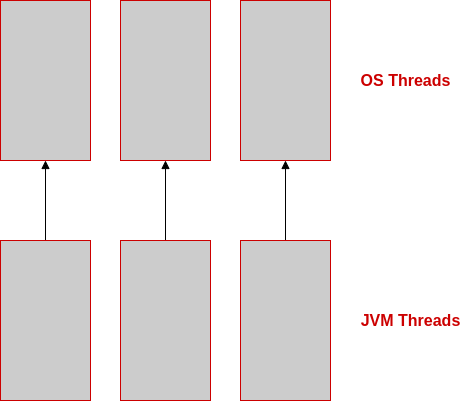
\includegraphics[width=0.9\textwidth]{img/jvm-threads.png}
            \label{JVM threads mapping.}
        \end{figure}
    \end{column}
    \begin{column}{.35\textwidth}
      \begin{block}{\centering Thread massimi}
        \vspace{2mm}
        \centering{\Large{10.000}}
        \vspace{2mm}
      \end{block}
      \vspace{4.5mm}
      \begin{block}{Dificoltà a scalare}
        \begin{itemize}
          \item \textit{shutdown esplicito}
          \item \textit{context switching}
          \item \textit{stack preallocato}
        \end{itemize}
      \end{block}
    \end{column}
  \end{columns}

\end{frame}

\begin{frame}[fragile]{Il Modello Fiber II}

  \begin{columns}
    \begin{column}{.6\textwidth}
      \begin{figure}
        \centering
            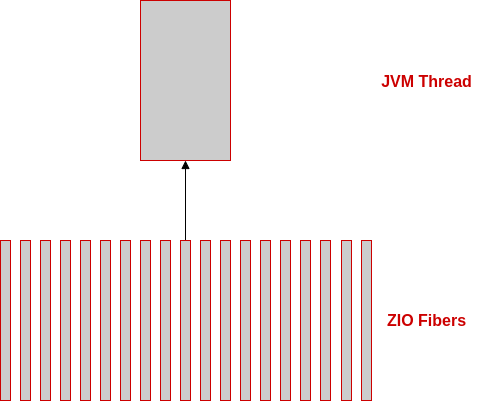
\includegraphics[width=0.9\textwidth]{img/fibers.png}
            \label{Fibers mapping.}
        \end{figure}
    \end{column}
    \begin{column}{.35\textwidth}
      \begin{block}{\centering Fiber massime}
        \vspace{2mm}
        \centering{\Large{1.000.000}}
        \vspace{2mm}
      \end{block}
      \vspace{4.5mm}
      \begin{block}{Elevata scalabilità}
        \begin{itemize}
          \item tipo componibile
          \item \textit{garbage collected}
          \item tempo di CS ridotto
          \item \textit{stack} dinamico
          \item supervisione
        \end{itemize}
      \end{block}
    \end{column}
  \end{columns}

\end{frame}

\begin{frame}{Interruzione}
  \begin{block}{ZIO Runtime}
    Nel caso in cui un \textit{effect} fosse seguito da un'interruzione e il suo risultato fosse inutilizzato, il \textit{runtime} di \texttt{ZIO} può decidere di non eseguirlo:
    \begin{itemize}
      \item ogni parte di un \textit{effect} può essere interrompibile
      \begin{itemize}
        \item fanno eccezione blocchi di codice importato affetti da \textit{side effect};
      \end{itemize}
      \item l'interruzione attende l'esecuzione di eventuali \textit{finalizer} (\texttt{ensuring});
    \end{itemize}
  \end{block}
  \begin{block}{Esempio: semplice interruzione}
    \lstinputlisting[language=Scala]{code/4a-interruzione.scala}    
  \end{block}
\end{frame}

\begin{frame}{Strutture Concorrenti}
  \begin{block}{Ref - Condivisione di stato}
    Per permette a più \textit{fiber} di condividere informazioni, \texttt{ZIO} fornisce la struttura \texttt{Ref}. Questa descrive una modifica di stato:
    \begin{itemize}
      \item alternativa puramente funzionale dell'\texttt{AtomicReference};
      \item le operazioni di accesso e modifica sono atomiche (\textit{safe}).
    \end{itemize}
  \end{block}
  \begin{block}{Esempio: modellazione di un contatore}
    \lstinputlisting[language=Scala]{code/4b-contatore.scala}    
  \end{block}
\end{frame}

\begin{frame}{Strutture Concorrenti II}
  \begin{block}{Queue - Distribuzione del lavoro}
    Una \texttt{Queue} consente di gestire molteplici valori distribuibili tra più \textit{fiber}.
     \begin{itemize}
      \item le operazioni fondamentali sono \texttt{offer} e \texttt{take};
      \item le possibili tipologie sono \texttt{unbounded} e \texttt{bounded};
      \item le strategie di inserimento sono \textit{Back pressure}, \textit{Sliding} e \textit{Dropping}.
     \end{itemize}
  \end{block}
  
  \begin{figure}
    \centering
    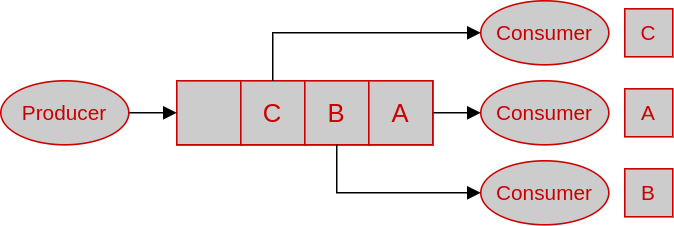
\includegraphics[width=0.7\textwidth]{img/queue.png}
    \label{distributing with queue.}
  \end{figure}

  % \begin{block}{Esempio: ping-pong con \texttt{bounded Queue}}
  %   \lstinputlisting[language=Scala]{code/4c-pingpong.scala}    
  % \end{block}

\end{frame}

\begin{frame}{Strutture Concorrenti III}
  \begin{block}{Hub - Broadcasting}
    La struttura \texttt{Hub} realizza un \textit{broadcasting} di informazioni:
    \begin{itemize}
      \item le operazioni fondamentali sono \texttt{publish} e \texttt{subscribe};
      \item le possibili tipologie sono \texttt{unbounded} e \texttt{bounded};
      \item le strategie di inserimento sono \textit{Back pressure}, \textit{Sliding} e \textit{Dropping}.
    \end{itemize}
  \end{block}
  \begin{figure}
    \centering
    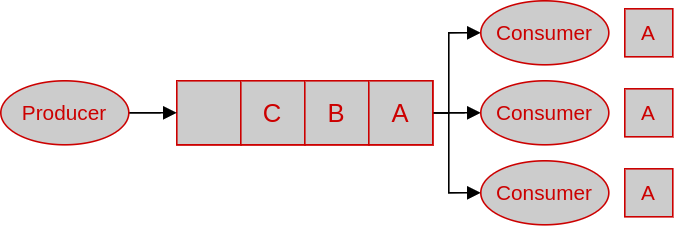
\includegraphics[width=0.7\textwidth]{img/hub.png}
    \label{broadcasting with hub.}
  \end{figure}
\end{frame}

